%%%%%%%%%%%%%%%%%%%%%%%%%%%%%%%%%%%%%%%%%%%%%%
% Head matter - can we try to be consistent on
% included packages
\ifdefined\beamerclass
\else
    \def\beamerclass{beamer}
\fi
\documentclass[\beamerclass]{beamer}

\usepackage{pgfpages}
\mode<handout>{
	% \setbeamercolor{background canvas}{bg=black!20}
	\pgfpagesuselayout{2 on 1}[a4paper,border shrink=5mm]
}

%\documentclass{beamer}
\mode<presentation>
{\usetheme{default}
 \usecolortheme{default}
 \usefonttheme{default}
 \setbeamertemplate{navigation symbols}{}
 \setbeamertemplate{footline}[frame number]
% \setbeamertemplate{caption}[numbered]
 }
\usepackage[english]{babel}
\usepackage{algorithm}
\usepackage[noend]{algpseudocode}
\usepackage[utf8x]{inputenc}
\usepackage{graphicx}
\usepackage{hyperref}
%\graphicspath{{./images/}}
\usepackage{tikz}
\usetikzlibrary{shapes.geometric, arrows,chains}
\usepackage{booktabs,makecell,multirow,tabularx}
\usepackage{verbatim}
\renewcommand{\arraystretch}{1.2}
\renewcommand\theadfont{\normalfont\bfseries}
\usepackage{array}
\usepackage{listings}
\lstset{language=Java, showstringspaces=false}
\usepackage[normalem]{ulem}
\usepackage{bm}
\def\layersep{2.5cm}

\usepackage{xcolor}
%\usepackage{subfig}
\setbeamertemplate{caption}{\insertcaption}
\usepackage[caption=false]{subfig}
\usepackage{hyperref}
\usepackage{verbatim}
%\setbeamertemplate{caption}[numbered]%\numberwithin{figure}{section}
% Define block styles
\tikzstyle{decision} = [diamond, draw, fill=blue!20, 
    text width=4.5em, text badly centered, node distance=3cm, inner sep=0pt]
\tikzstyle{block} = [rectangle, draw, fill=blue!20, 
    text width=3em, text centered, rounded corners, minimum height=3em]
\tikzstyle{line} = [draw, -latex']
\tikzstyle{cloud} = [draw, ellipse, fill=red!20, node distance=3cm,
    minimum height=2em]
\tikzset{
  startstop/.style={
    rectangle, 
    rounded corners,
    minimum width=3cm, 
    minimum height=1cm,
    align=center, 
    draw=black, 
    fill=red!30
    },
  process/.style={
    rectangle, 
    minimum width=3cm, 
    minimum height=1cm, 
    align=center, 
    draw=black, 
    fill=blue!30
    },
  decision/.style={
    rectangle, 
    minimum width=3cm, 
    minimum height=1cm, align=center, 
    draw=black, 
    fill=green!30
    },
  arrow/.style={thick,->,>=stealth},
  dec/.style={
    ellipse, 
    align=center, 
    draw=black, 
    fill=green!30
    },
}
\tikzstyle{arrow} = [thick,->,>=stealth]

\tikzset{onslide/.code args={<#1>#2}{%
  \only<#1>{\pgfkeysalso{#2}} % \pgfkeysalso doesn't change the path
}}

\makeatletter
\newenvironment<>{btHighlight}[1][]
{\begin{onlyenv}#2\begingroup\tikzset{bt@Highlight@par/.style={#1}}\begin{lrbox}{\@tempboxa}}
{\end{lrbox}\bt@HL@box[bt@Highlight@par]{\@tempboxa}\endgroup\end{onlyenv}}

\newcommand<>\btHL[1][]{%
  \only#2{\begin{btHighlight}[#1]\bgroup\aftergroup\bt@HL@endenv}%
}
\def\bt@HL@endenv{%
  \end{btHighlight}%   
  \egroup
}
\newcommand{\bt@HL@box}[2][]{%
  \tikz[#1]{%
    \pgfpathrectangle{\pgfpoint{1pt}{0pt}}{\pgfpoint{\wd #2}{\ht #2}}%
    \pgfusepath{use as bounding box}%
    \node[anchor=base west, fill=orange!30,outer sep=0pt,inner xsep=1pt, inner ysep=0pt, rounded corners=3pt, minimum height=\ht\strutbox+1pt,#1]{\raisebox{1pt}{\strut}\strut\usebox{#2}};
  }%
}
\makeatother




%%%%%%%%%%%%%%%%%%%%%%%%%%%%%%%%%%%%%%%%%%%%%%
% Formatting for title page
\title[Deep Learning]{Recurrent Neural Networks}
\author{Kate Farrahi}
\institute{ECS Southampton}
\date{\today}
%%%%%%%%%%%%%%%%%%%%%%%%%%%%%%%%%%%%%%%%%%%%%%
\begin{document}
\begin{frame}
  \titlepage
\end{frame}
%-------------------------------------------------------------%


\begin{frame}[fragile]{pause}\frametitle{Batch Normalization}
\begin{itemize}
\item Batch normalization (BN) is a technique for improving the performance of ANNs
\item It improves the stability of ANNs by adjusting and scaling the activations
\item BN makes your ANN more robust to the choice of hyperparameters (larger range of parameters that will work well)
\item It was introduced by Sergey Ioffe and Christian Szegedy in 2015 \footnote{\url{https://arxiv.org/pdf/1502.03167.pdf}}
\end{itemize}
\end{frame}
%-------------------------------------------------------------%

\begin{frame}[fragile]{pause}\frametitle{Batch Normalization}
\center{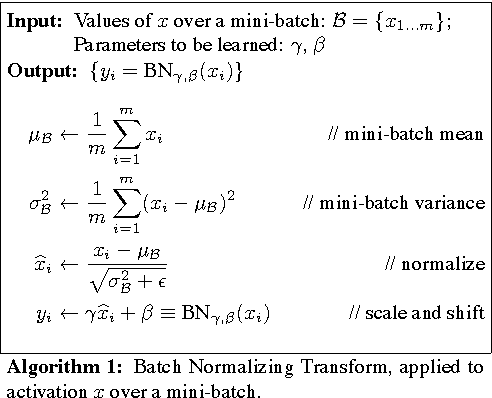
\includegraphics[width=0.9\textwidth]{batchnorm.pdf}}
\end{frame}
%-------------------------------------------------------------%

\begin{frame}[fragile]{pause}\frametitle{Batch Normalization}
\center{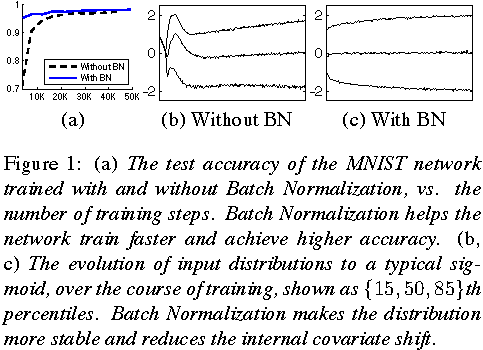
\includegraphics[width=0.9\textwidth]{BN_fig1.pdf}}
\end{frame}
%-------------------------------------------------------------%

\begin{frame}[fragile]{pause}\frametitle{Batch Normalization}
\center{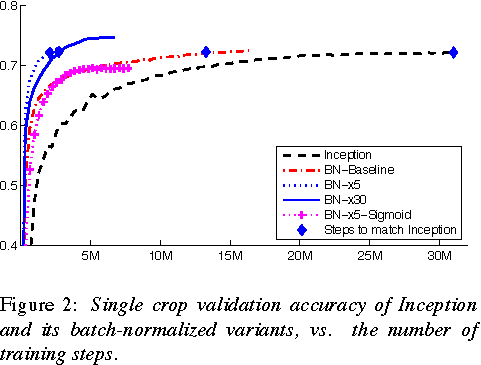
\includegraphics[width=0.9\textwidth]{BN_fig2.pdf}}
\end{frame}
%-------------------------------------------------------------%

\begin{frame}[fragile]{pause}\frametitle{Recurrent Neural Networks - Motivation}
\begin{center}
\begin{tabular}{ c c c c c c c c c}
$x$: & Kate & Farrahi & and & Jonathon & Hare & teach & deep & learning \\ \\
$y$: & 1 & 1 & 0 & 1 & 1 & 0 & 0 & 0 \\
\end{tabular}
\end{center}
\end{frame}
%-------------------------------------------------------------%

\begin{frame}[fragile]{pause}\frametitle{Recurrent Neural Networks - Motivation}
\begin{center}
\begin{tabular}{ c c c c c c c }
$x$: & $x^{<1>}$ & $x^{<2>}$ & ... & $x^{<t>}$ & ... &$x^{<T_x>}$ \\
$x$: & Kate & Farrahi & ... & Hare &... & learning \\ \\
$y$: & $y^{<1>}$ & $y^{<2>}$ & ... & $y^{<t>}$ & ... &$y^{<T_y>}$ \\
$y$: & 1 & 1 & ... & 1 & ...& 0 \\ \\ \\
\end{tabular}
\end{center}

In this example, $T_x = T_y = 8$ but $T_x$ and $T_y$ can be different.
\end{frame}
%-------------------------------------------------------------%


\begin{frame}[fragile]\frametitle{One Hot Encoding}

How can we represent individual words?
\center{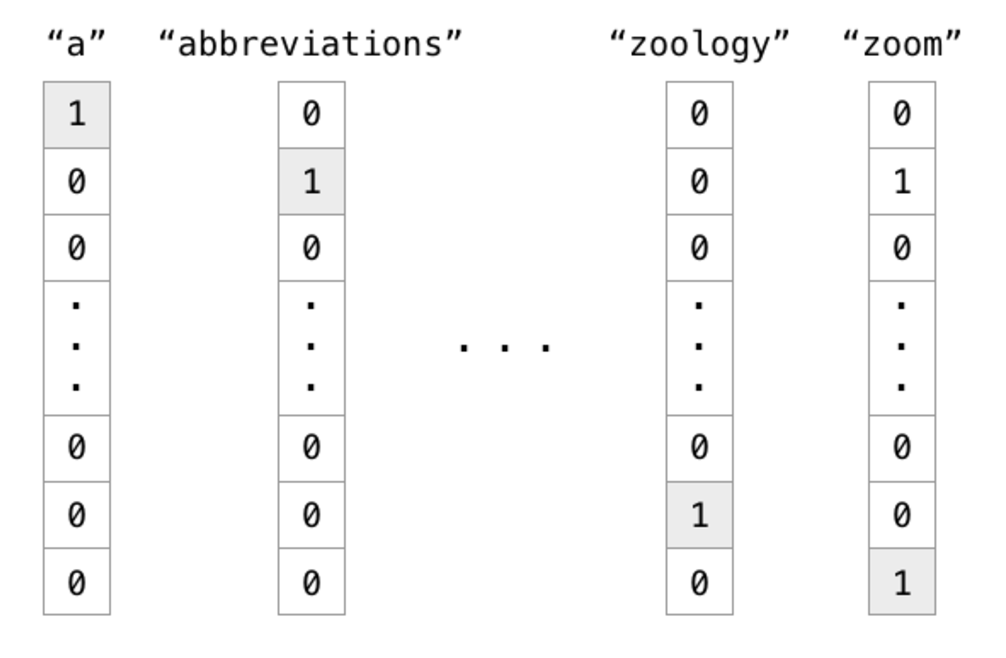
\includegraphics[width=0.9\textwidth]{onehot.pdf}\footnote{\url{https://ayearofai.com}}}
\end{frame}
%-------------------------------------------------------------%

\begin{frame}[fragile]{pause}\frametitle{Why Not a Standard Feed Forward Network?}
\begin{itemize}
\item For a task such as "Named Entity Recognition" a feed forward network would have several disadvantages \pause
\item The inputs and outputs may have varying lengths \pause
\item The features wouldn't be shared across different positions in the network
\end{itemize}
\end{frame}
%-------------------------------------------------------------%

\begin{frame}[fragile]{pause}\frametitle{Recurrent Neural Networks}
\center{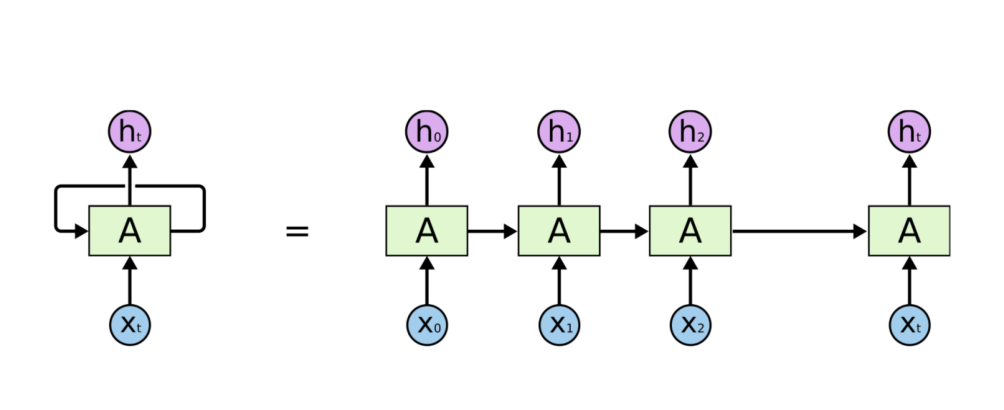
\includegraphics[width=0.99\textwidth]{rnn1.pdf}\footnote{Image taken from \url{https://towardsdatascience.com}}}
\begin{itemize}
\item RNNs are a family of ANNs for processing sequential data \pause
\item RNNs have directed cycles in their computational graphs \pause
\item They can have complicated dynamics, difficult to train \pause
\item They are more biologically realistic 
\end{itemize}
\end{frame}
%-------------------------------------------------------------%

\begin{frame}[fragile]\frametitle{Recurrent Neural Networks}
%\center{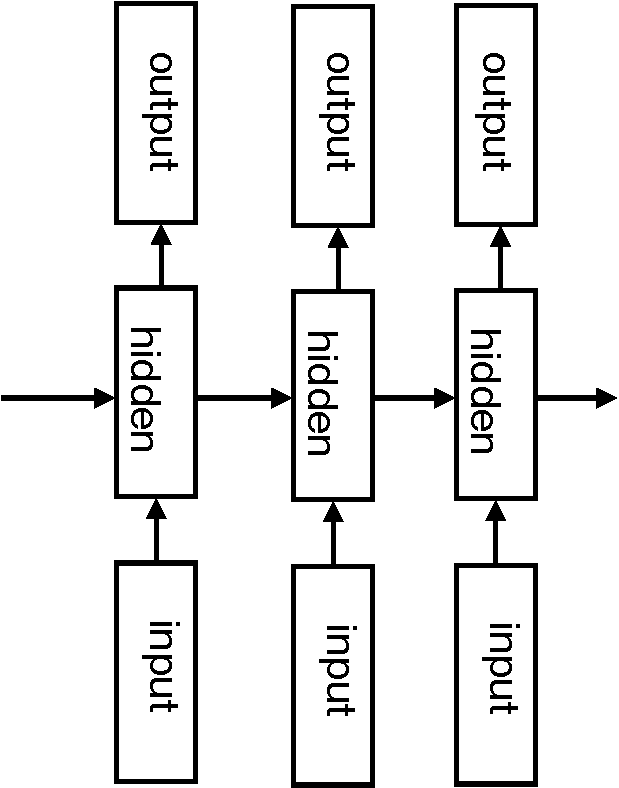
\includegraphics[width=0.3\textwidth]{RNN.pdf}} 
RNNs combine two properties which make them very powerful.
\begin{enumerate}
\item Distributed hidden state that allows them to store a lot of information about the past efficiently. This is because several different units can be active at once, allowing them to remember several things at once.
\item Non-linear dynamics that allows them to update their hidden state in complicated ways. They can however have complicated dynamics, making them difficult to train
\end{enumerate}

\end{frame}
%-------------------------------------------------------------%

\begin{frame}[fragile]\frametitle{Backpropagation Through Time (BPTT)}
\center{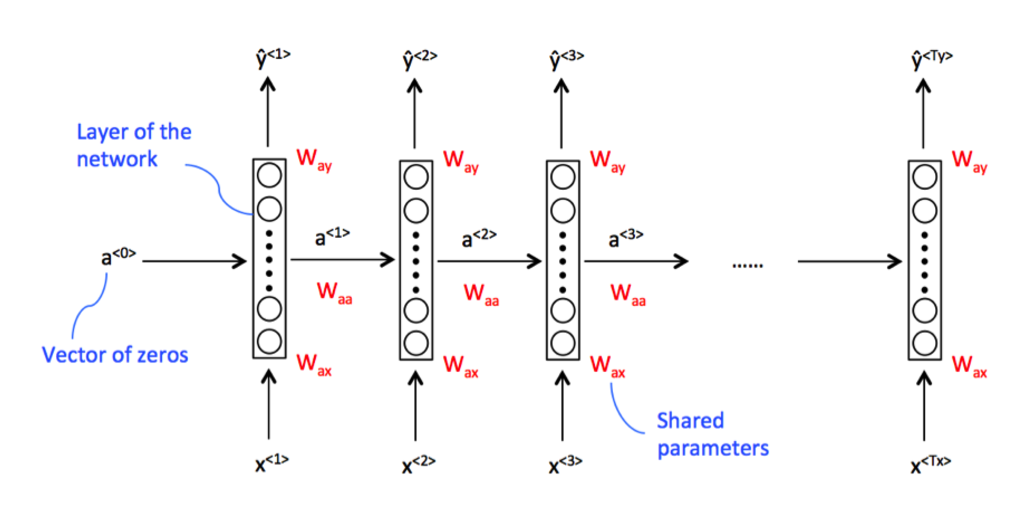
\includegraphics[width=0.99\textwidth]{rnn_ng.pdf}\footnote{Image taken from Andrew Ng}}
\end{frame}
%-------------------------------------------------------------%

\begin{frame}[fragile]{pause}\frametitle{BPTT - Forward Pass}
\begin{eqnarray}
a^{<t>} &=& g(w_{aa} a^{<t-1>} + w_{ax} x^{<t>} + b_a) \\ \pause
\hat y^{<t>} &=& g(w_{ya} a^{<t>} + b_y) \\ \pause
\mathcal{L}^{<t>} &=& -y^{<t>} log(\hat y^{<t>}) - (1 - y^{<t>}) log(1 - \hat y^{<t>}) \\ \pause
\mathcal{L} &=& \sum_{t = 1}^{T_y} \mathcal{L}^{<t>}
\end{eqnarray}
\end{frame}
%-------------------------------------------------------------%

\begin{frame}[fragile]{pause}\frametitle{BPTT - Backwards Pass}
\begin{eqnarray}
\frac{\partial \mathcal{L}^{<3>}}{\partial w_{ya}} &=&  \frac{\partial \mathcal{L}^{<3>}}{\partial \hat y^{<3>}} \frac{\partial \hat y^{<3>}}{\partial w_{ya}}\\ \pause
\frac{\partial \mathcal{L}^{<3>}}{\partial w_{aa}} &=&  \frac{\partial \mathcal{L}^{<3>}}{\partial \hat y^{<3>}} \frac{\partial \hat y^{<3>}}{\partial a^{<3>}} \frac{\partial \hat a^{<3>}}{\partial w_{aa}}\\\\ \pause
\text{Recall } a^{<3>} & = & g(w_{aa} a^{<2>} + w_{ax} x^{<3>} + b_a) \nonumber \\
\frac{\partial \mathcal{L}^{<3>}}{\partial w_{aa}} &=& \frac{\partial \mathcal{L}^{<3>}}{\partial \hat y^{<3>}} \frac{\partial \hat y^{<3>}}{\partial a^{<3>}} \frac{\partial a^{<3>}}{\partial a^{<2>}}\frac{\partial a^{<2>}}{\partial a^{<1>}}\frac{\partial a^{<1>}}{\partial w_{aa}}
\end{eqnarray}
\end{frame}
%-------------------------------------------------------------%

\begin{frame}[fragile]\frametitle{Recurrent Neural Networks}
\center{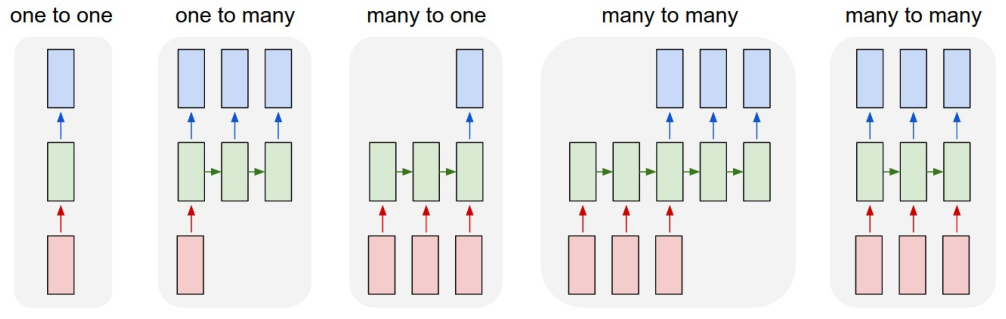
\includegraphics[width=0.99\textwidth]{seqmods.pdf}}  \footnote{\url{http://karpathy.github.io/2015/05/21/rnn-effectiveness/}}
\end{frame}
%-------------------------------------------------------------%


%\begin{frame}[fragile]\frametitle{Recurrent Neural Networks for Modeling Sequences}
%\center{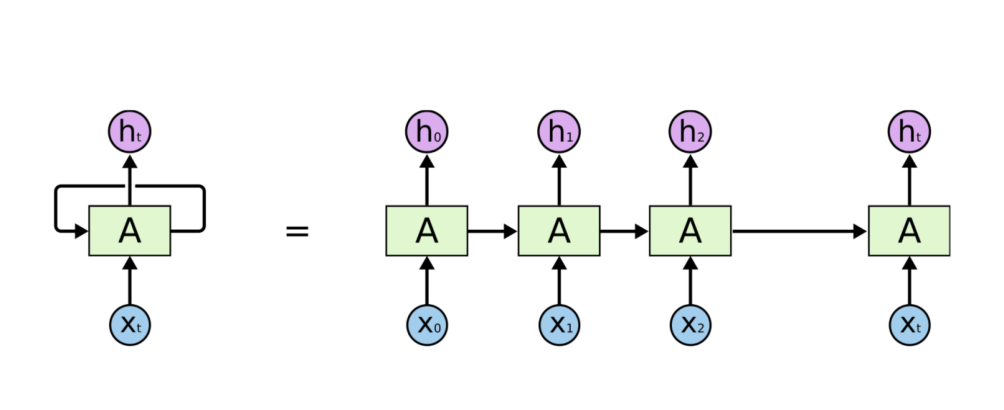
\includegraphics[width=0.99\textwidth]{rnn1.pdf}} 
%\begin{eqnarray}
%h_t &=& f_W(h_{t-1}, x_t)\\
%h_t &=& tanh(W_{hh} h_{t-1} + W_{xh} x_t)\\
%y_t &=& W_{hy} h_t
%\end{eqnarray}
%\begin{itemize}
%\item Recurrent Neural Networks are a very natural way to model sequential data
%\item They are equivalent to very deep networks with one hidden layer per time slice
%\end{itemize}
%\end{frame}
%-------------------------------------------------------------%
%
%\begin{frame}[fragile]\frametitle{RNN Based Language Model}
%\begin{itemize}
%\item The first paper to investigate the use of RNNs for modeling sequential data applied to speech recognition \footnote{Mikolov, Tomas, et al. "Recurrent neural network based language model." Eleventh annual conference of the international speech communication association. 2010.}.
%\item Previous work \footnote{Bengio, Yoshua, et al. "A neural probabilistic language model." Journal of machine learning research 3.Feb (2003): 1137-1155.} used a Feedforward NN with fixed length context that needs to be specified before training.
%\item They train a network with $30-500$ hidden units using standard backpropagation with SGD.
%\end{itemize}
%\end{frame}
%%-------------------------------------------------------------%
%
%\begin{frame}[fragile]\frametitle{RNN Based Language Model Architecture}
%\center{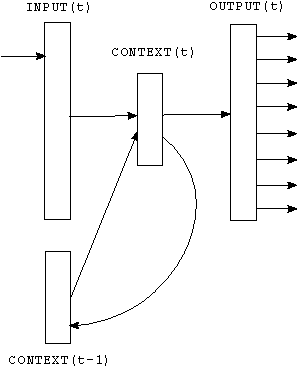
\includegraphics[width=0.3\textwidth]{mikolov.pdf}}
%\begin{eqnarray}
%x(t) &=& w(t) + s(t-1)\\
%s_j(t) &=& f(\sum_i x_i(t) u_{ji}) \text{, where $f$ is a sigmoid function}\\
%y_k(t) &=& g(\sum_j s_j(t) v_{kj})  \text{, where $g$ is a softmax function}
%\end{eqnarray}
%\end{frame}
%%-------------------------------------------------------------%
%
%\begin{frame}[fragile]\frametitle{Speech Recognition with Deep Recurrent Neural Networks}
%\end{frame}
%%-------------------------------------------------------------%

\end{document}
